\documentclass[12pt,]{article}

\usepackage[svgnames,table]{xcolor}
\usepackage{mathtools}
\usepackage[italian]{babel}
\usepackage{graphicx}
\usepackage[utf8]{inputenc}
\usepackage{float}
\usepackage{tabularx}
\usepackage{chngpage}
\usepackage[toc,page]{appendix}
\usepackage{gensymb}
\usepackage{subcaption}
\usepackage{tikz}
\usepackage{circuitikz}
\usepackage{array}
\usepackage{booktabs} 
\usepackage{colortbl} 
\usepackage{xcolor} 
\usepackage{xfrac}


\definecolor{burntorange}{cmyk}{0, 0.51,1,0}


\begin{document}
 \begin{titlepage}

\newcommand{\HRule}{\rule{\linewidth}{0.5mm}} % Defines a new command for the horizontal lines, change thickness here

\center % Center everything on the page
 
%----------------------------------------------------------------------------------------
%	HEADING SECTIONS
%----------------------------------------------------------------------------------------

\includegraphics[width = 50mm]{unitn.jpg}\\[0.5cm]
\textsc{\LARGE Università degli studi di Trento}\\[1.5cm] % Name of your university/college
\textsc{\Large Laboratorio di fisica II}\\[0.5cm] % Major heading such as course name
\textsc{\large Esperienza 2-3}\\[0.5cm] % Minor heading such as course title

%----------------------------------------------------------------------------------------
%	TITLE SECTION
%----------------------------------------------------------------------------------------

\HRule \\[0.2cm]
{ \huge \bfseries CIRCUITO RC E\\[0.1cm]FILTRI PASSA BASSO-ALTO}\\ % Title of your document
\HRule \\[1.5cm]
 
%----------------------------------------------------------------------------------------
%	AUTHOR SECTION
%----------------------------------------------------------------------------------------

\begin{minipage}{0.4\textwidth}
\begin{flushleft} \large
\emph{Autori:}\\
Canteri Marco\\Biasi Lorenzo\\Damiani Emily % Your name
\end{flushleft}
\end{minipage}
~
\begin{minipage}{0.4\textwidth}
\begin{flushright} \large
\emph{Professore:} \\
William J. Weber % Supervisor's Name
\end{flushright}
\end{minipage}\\[1.5cm]

% If you don't want a supervisor, uncomment the two lines below and remove the section above
%\Large \emph{Author:}\\
%John \textsc{Smith}\\[3cm] % Your name

%----------------------------------------------------------------------------------------
%	DATE SECTION
%----------------------------------------------------------------------------------------

{\large \today}\\[3cm] % Date, change the \today to a set date if you want to be precise

%----------------------------------------------------------------------------------------
%	LOGO SECTION
%----------------------------------------------------------------------------------------

%\includegraphics{Logo}\\[1cm] % Include a department/university logo - this will require the graphicx package
 
%----------------------------------------------------------------------------------------

\vfill % Fill the rest of the page with whitespace

\end{titlepage}

	\newpage
	\renewcommand{\abstractname}{Abstract}

	\begin{abstract}
In questa esperienza si è realizzato il Ponte di Wien con un condensatore dal valore incognito. Per farne una misura si sono realizzate le condizioni per il bilanciamento del ponte. In un secondo momento, si è studiato la risposta del circuito a piccoli cambiamenti di capacità. In questo modo si è potuto quantificare con quale precisione il circuito risponde alla più piccola variazione di capacità apprezzabile. 

	\end{abstract}
  \vspace{10em}
\tableofcontents
  \newpage
  \section{Obiettivi}
  \begin{itemize}
  \item realizzare il ponte di Wien, utilizzando una capacità dal valore incognito, e ottenere le condizioni di bilanciamento del ponte. 
  \item confrontare il valore della capacità ottenuto teoricamente dalle condizioni di bilanciamento con il valore registrato dal multimetro digitale. 
  \item studiare come variano i valori di tensione in uscita dal circuito per  piccole variazioni della capacità. 
  \item quantificare con quanta precisione lo strumento reagisce a piccole variazioni di capacità. 
  \end{itemize}
  
\section{Materiali}
\begin{itemize}
\item breadbord
\item cavi coassiali 
\item 3 resistenze misurate con il multimetro digitale
\item 2 capacità
\item generatore di onda sinusoidale 
\item decade di capacità
\item decade di resistenza  
\item Oscilloscopio 
\end{itemize}
\section{Procedura di misura}
Nella prima parte dell'esperienza si è misurato il valore della capacità di un condensatore incognito $C_x$. Per fare ciò si è costruito il circuito mostrato in figura \eqref{fig:circuito}, chiamato Ponte di Wien. 
Al circuito è stato collegato l'oscilloscopio in modalità \emph{math} con numero di medie pari a 8, per la misura di $V_{out}$. Abbiamo bilanciato poi il ponte, cercando i valori di frequenza e di resistenza $R_r$ che danno un uscita del ponte il più possibile nulla.\\ Dalle condizioni di bilanciamento siamo risaliti al valore della capacità $C_x$.
Per misurare la sensibilità del circuito abbiamo fatto piccole variazioni di $C_x$ con una scatola decade di capacità in parallelo e in serie a $C_x$. Per ogni variazione si sono prese 10 misure.
\begin{table}[H]
\centering
\begin{tabular}{c|c}
\toprule 
\multicolumn{2}{c}{Resistenze del ponte}\\
\midrule
$R_1$ &  $1007.2\pm 11.0720 \ohm$   \\
$R_2$ &  $997.80\pm 10.9780 \ohm$  \\
$R_x$ & $999.021 \pm 10.9902 \ohm$  \\
$C_2$ & $112 \pm 5.48 \text{ nF}$ \\
\bottomrule
\end{tabular}
\caption{Valori misurati con il multimetro digitale}
\end{table}

\begin{figure}[H]
\centering
\begin{circuitikz}
\draw (0,0)
to [sV= $ V_{in}$] (0,6)
to [short] (5,6)
to [short] (5,5.5)
to[short] (2.5,5.5)
to [vR= $ R_r $] (2.5,3)
to [short] (1.5, 3)
to[R=$ R_x $] (1.5, 0.75)
to[short](2.5, 0.75)
to[short](2.5,0.5)
;
\draw (2.5, 3)
to[short](3.5,3)
to[C=$ C_x$] (3.5, 0.75)
to[short] (2.5, 0.75)
;
\draw (5, 5.5)
to[short](7, 5.5)
to[R=$ R_1 $](7, 3)
to[R= $ R_2 $] (7, 1.5)
to[C= $ C_2 $] (7, 0.5)
to[short](7, 0.5)
to[short] (2.5, 0.5)
;
\draw (4.75, 0.5)
to[short] (4.75, 0)
to[short](0,0)
;
\draw (2.5, 3.5)
to[short, -o](4, 3.5)node[right = 0.5em] {$V_{out}$}
;
\draw (7, 3.5)
to[short, -o](5.5, 3.5)
;
\end{circuitikz}

\caption{Circuito utilizzato, ponte di Wien}
\label{fig:circuito}
\end{figure}

\section{Analisi ponte bilanciato}
\begin{figure}[H]
\centering
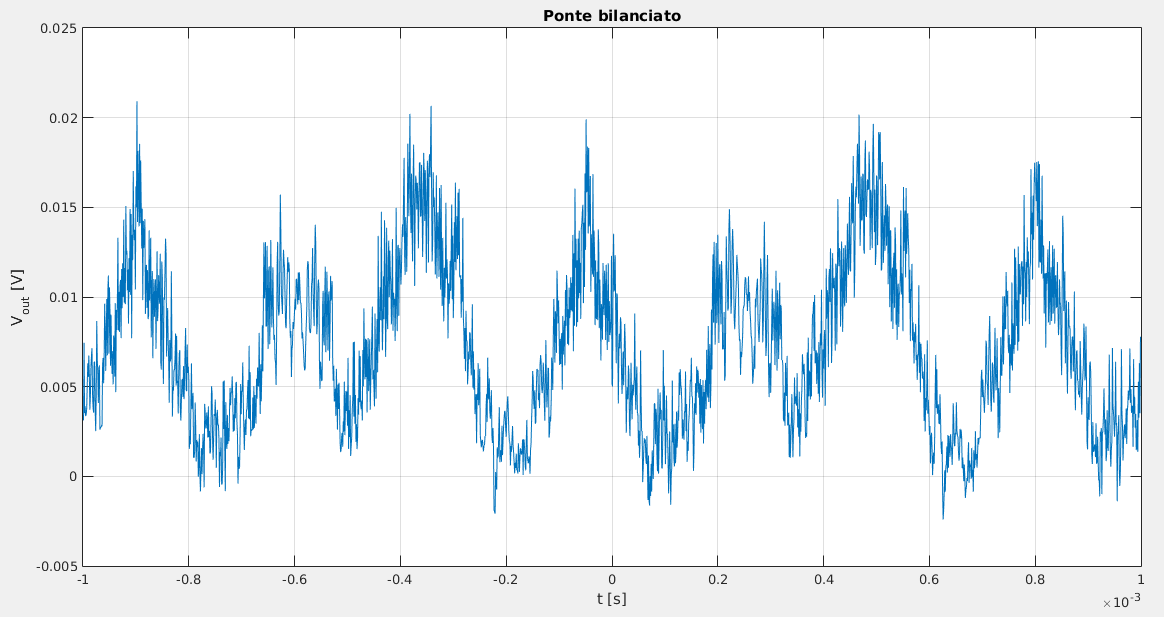
\includegraphics[width=\textwidth]{pontebilanciato}
\caption{Uscita del ponte bilanciato al meglio delle nostre possibilità}
\end{figure}
Per ottenere le condizioni di bilanciamento, ovvero $V_{out}=0$, bisogna soddisfare le seguenti equazioni: 
 \begin{equation}
 \frac{R_2}{R_x} + \frac{C_x}{C_2} = \frac{R_1}{R_r}
 \end{equation}
 \begin{equation}
 \omega^2 R_2  C_2  R_x  C_x = 1 
 \end{equation}
Trovata la condizione di bilanciamento possiamo ricavare il valore della capacità $C_x$ a partire da queste due equazioni: 
\begin{equation}
\label{eq:cx}
C_x = \sqrt{\frac{1}{\omega^2 R_2 R_x} \biggl(\frac{R_1}{R_r} - \frac{R_2}{R_x} \biggr)}
\end{equation}
\begin{table}[H]
\centering
\begin{tabular}{c|c}
\toprule
\multicolumn{2}{c}{Valori per il bilanciamento del ponte}\\
\midrule
\rowcolor{black!20}$R_r$ & $430 \pm 4.3  \ohm$ \\
$f$ & $ 1178.24\pm 0.5 Hz $ \\
\rowcolor{black!20}$C_x$ & $156.82 \pm 3.6349 nF $ \\
\bottomrule
\end{tabular}
\caption{Valori di bilanciamento e $C_x$ ricavato, con $f = \omega/2\pi$}
\end{table}
L'incertezza su $C_x$ si ottiene propagando l'incertezza dall'equazione \eqref{eq:cx}

\section{Analisi sensibilità ponte}
L'uscita del ponte sbilanciato segue una legge del tipo
\begin{equation}
\label{eq:gen}
V_{out} = V_c\, sin(\omega t + \phi) + V_r\, cos(\omega t + \phi)
\end{equation}
Dove le ampiezza $V_c$ e $V_r$ dipendono rispettivamente da una variazione lineare di $C_x$ e di $R_x$ per valori vicini alla condizione di bilanciamento: $V_c = (\partial V_c/\partial C_x) \Delta C_x$. Sviluppandolo con le forme di addizione otteniamo
\begin{equation}
\label{eq:fit}
V_{out}=V_0 + V_{sin}\, sin (\omega t) + V_{cos} \,cos(\omega t)
\end{equation}
Dove abbiamo:
\begin{equation}
V_{sin} = V_c\, cos\phi -V_r\, sin\phi \qquad V_{cos} = V_c\, sin\phi + V_r\, cos\phi
\end{equation}
$V_0$ è stato aggiunto per eliminare un eventuale errore di offset. Possiamo ora fare il fit sui nostri dati con l'equazione \eqref{eq:fit}.
I valori di $V_{sin}$ e $V_{cos}$ sono stati calcolati come media dei 10 valori delle nostre misure, e come loro incertezza la deviazione standard.
\begin{figure}[H]
\centering
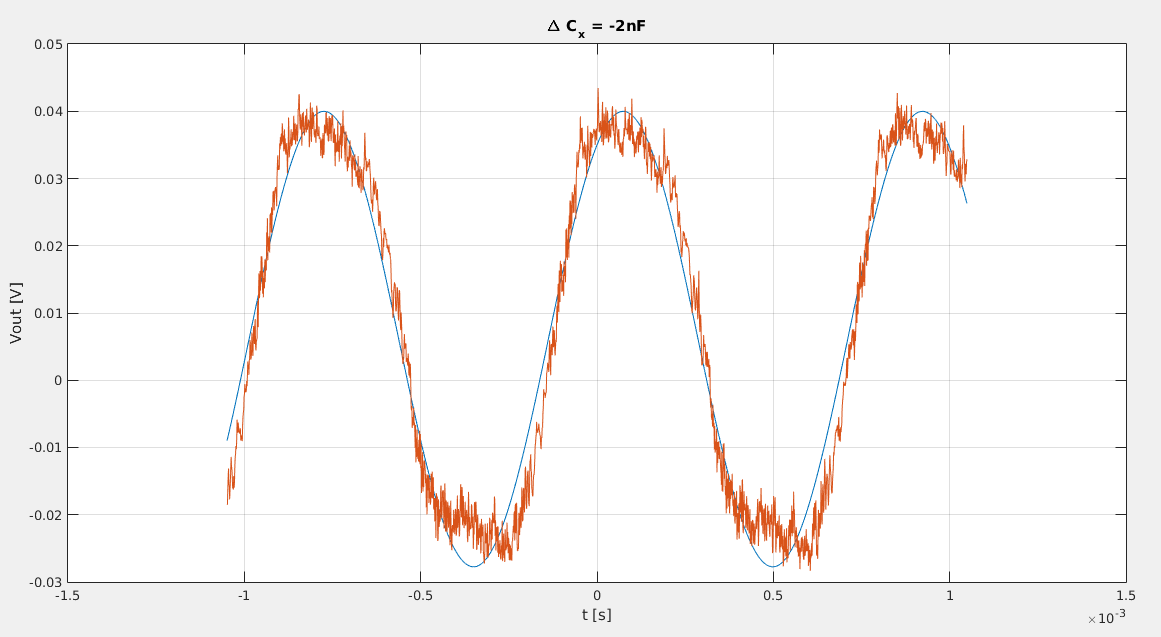
\includegraphics[width=\textwidth]{fit1}
\caption{Esempio fit dati $\Delta C_x$ negativo}
\end{figure}
\begin{figure}[H]
\centering
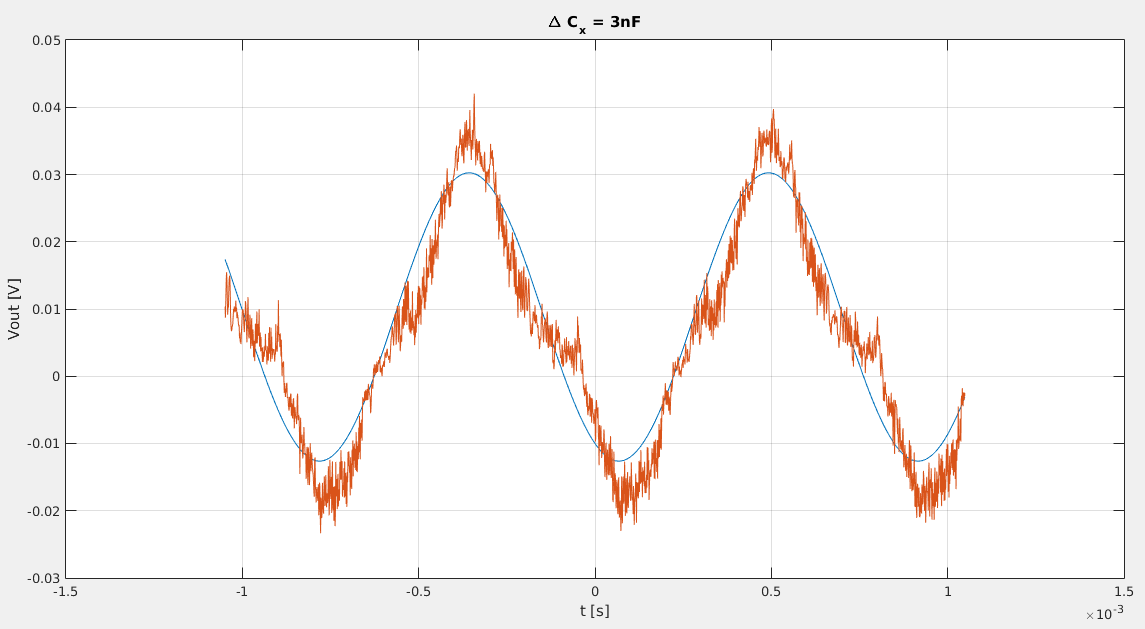
\includegraphics[width=\textwidth]{fit2}
\caption{Esempio fit dati $\Delta C_x$ positivo}
\end{figure}
Ora con una regressione lineare dei parametri appena trovati in funzione di $ \Delta C_x$.
$$V_{sin}= A_s + B_s \Delta{C_x}$$
$$V_{cos} = A_c + B_c \Delta{C_x}$$
Possiamo trovare 
\begin{equation}
\phi = \arctan{\frac{B_c}{B_s}}
\end{equation}
\begin{equation}
\frac{\partial{V_{c}}}{\partial{C_x}} = \sqrt{B_s^2 + B_c^2}
\end{equation}
\begin{figure}[H]
\centering
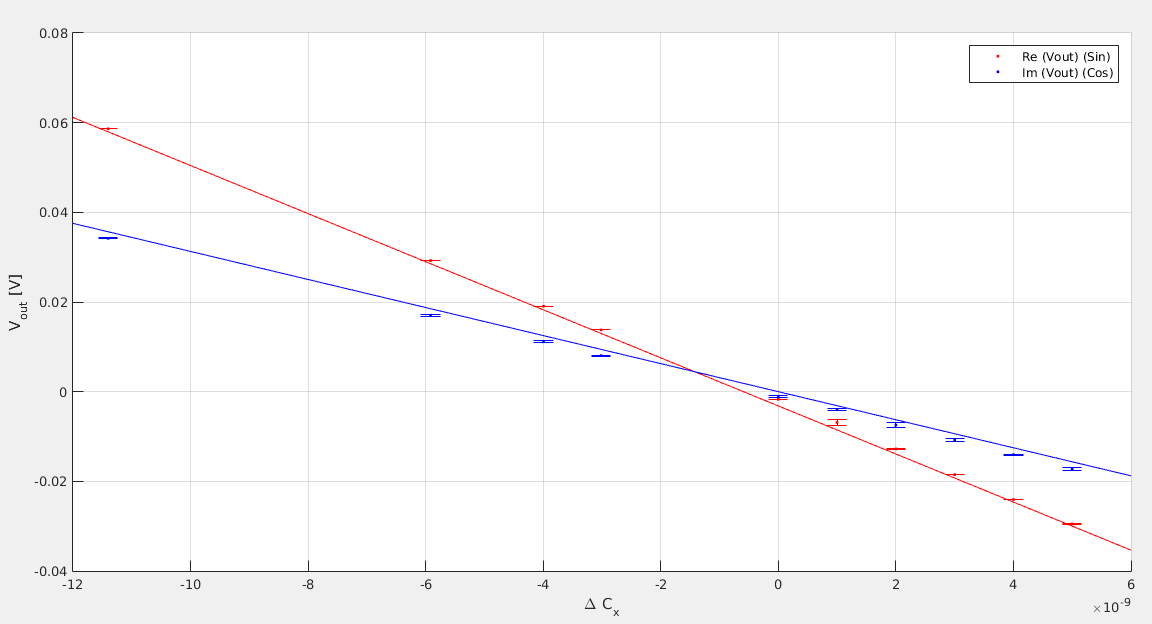
\includegraphics[width=\textwidth]{fitsensibilita}
\caption{Fit per la sensibilità}
\end{figure}
Dai nostri dati otteniamo
\begin{table}[H]
\centering
\begin{tabular}{c|c}
\toprule
\multicolumn{2}{c}{Valori ottenuti dal fit}\\
\midrule
\rowcolor{black!20}$\phi$ & $-120.2 \pm 0.1 \degree$ \\
$\partial V_{c}/\partial C_x $ & $ 6.207 10^{6}\pm 9.5 10^{3} V/F $ \\
\bottomrule
\end{tabular}
\caption{Risultati del fit}
\end{table}
Ora possiamo tornare all'equazione \eqref{eq:gen} e fare il fit con il valore di $\phi$ appena ricavato, in modo da ottenere $V_c$ e risalire alla variazione $\Delta C_m = V_c/(\partial V_{c}/\partial{C_x})$ misurata col ponte.
\begin{figure}[H]
\centering
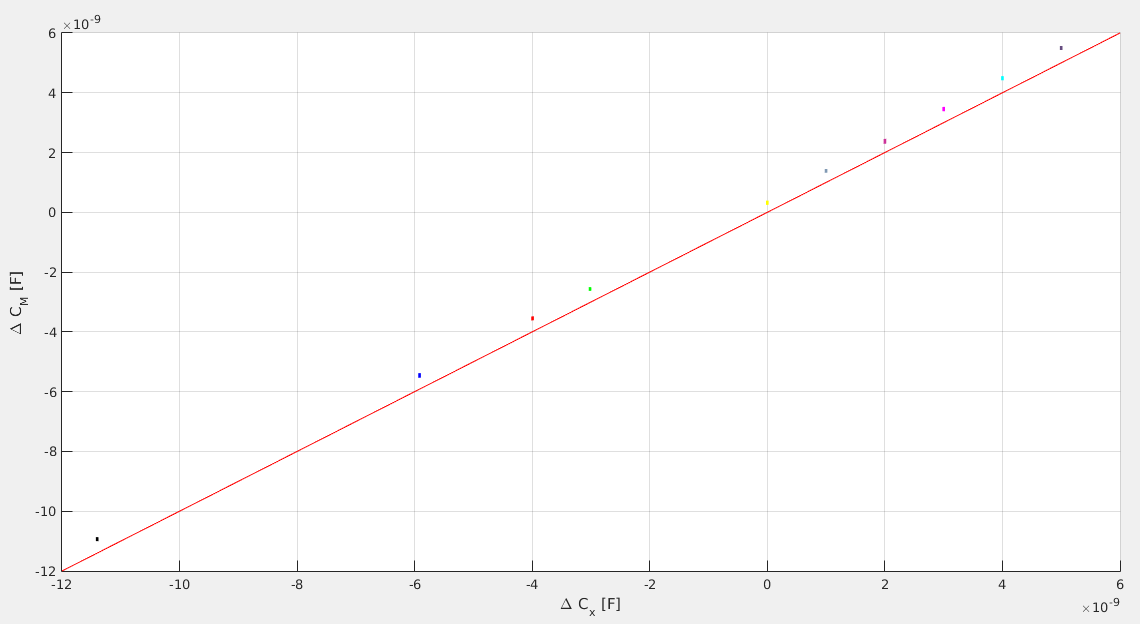
\includegraphics[width=\textwidth]{deltacm}
\caption{$\Delta C_m$ ricavati dall'analisi e $\Delta C_x$ che abbiamo variato}
\end{figure}
La retta tracciata $y=x$ è l'andamento teorico che dovremmo avere, ovvero la variazione che abbiamo fatto deve corrispodere alla variazione misurata dall'uscita del ponte ricavata tramite l'analisi appena fatta. L'incertezza su $\Delta C_m$ e di conseguenza la sensibilità del nostro ponte è stata calcolata con la deviazione standard su $\Delta C_m$.
\section{Conclusioni}
Dall'ultimo grafico è evidente che le variazioni di capacità misurate non corrispondono alle variazioni ricavate dall'analisi, l'andamento però è sistematico e si può spiegare con il fatto che il ponte che credevamo bilanciato in realtà non lo era. Lo si può anche notare dal grafico dove è stata rappresentata anche l'analisi dell'uscita del ponte bilanciato, ci ha fornito un $\Delta C_m$ non nullo. Lo sbilanciamento si può quantificare usando il grafico ed è di circa $0.1 \text{ nF}$. Bisogna notare quando abbiamo bilanciato il ponte, avevamo a disposizione una decade di resistenze con $\Delta R_r$ minimo di $1 \ohm$. Si può vedere utilizzando l'equazione \eqref{eq:cx}, che una variazione di un $\ohm$ risulta in una variazione di circa $0.32 \text{ nF}$ ovvero una quantità maggiore dell'errore che abbiamo commesso per il bilanciamento.\\
Bisogna inoltre notare che abbiamo trascurato la presenza dell'oscilloscopio nell'analisi, in quanto risultava trascurabile. Infatti nel circuito "vero" la resistenza e il condensatore dell'oscilloscopio sono in parallelo a $C_x$ e $R_x$: la resistenza e il condensatore equivalenti risultano diversi dai valori da noi usati per meno di $1 \%$. 
\end{document}
